% 第 22 题抛物线图：按固定源 PDF 矢量路径换算（1 pt → 0.03515 cm）。
% 原点取 O（抛物线顶点，源页 (1027.76, 234.91) pt），y 向上。
% 抛物线线宽 0.8pt（其余图元 2 倍），按源精确作图：单位长 14.168 pt、p=1 单位（y²=2px 逐点残差 ≤0.001）；
% 上下两支在 u=6.35 单位（x=89.96）处齐头收笔；直线 l 斜率页面 −1（数学 +1）、截距 ±2 单位，均照源。
% x 轴左 −28.34 右至箭头尖点 113.34；y 轴下 −70.84 上至箭头尖点 70.84；曲线名 C 标注在上支端头旁。
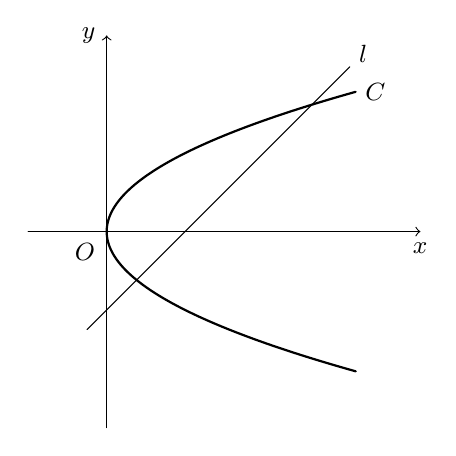
\begin{tikzpicture}[line cap=round,line join=round,font=\small,x=0.03515cm,y=0.03515cm]
% 坐标轴
\draw[->] (-28.34,0)--(113.34,0);
\draw[->] (0,-70.84)--(0,70.84);
% 抛物线（线宽 0.8，与源一致；单位长 14.168）
\draw[line width=0.8pt] plot[domain=-3.5636:3.5636,samples=121] ({(\x*\x/2)*14.168},{\x*14.168});
% 直线 l
\draw (-7.09,-35.42)--(87.84,59.50);
% ===== 标注（照源字框中心，显式坐标）=====
\node[anchor=center,inner sep=0] at (-6.50,70.84) {\(y\)};
\node[anchor=center,inner sep=0] at (92.69,64.37) {\(l\)};
\node[anchor=center,inner sep=0] at (97.08,50.49) {\(C\)};
\node[anchor=center,inner sep=0] at (-7.85,-7.28) {\(O\)};
\node[anchor=center,inner sep=0] at (113.26,-5.96) {\(x\)};
\end{tikzpicture}
